\documentclass{acm_proc_article-sp}
% \usepackage{fullpage}
\usepackage{amsmath}
\usepackage{amssymb}
\usepackage{proof}
\usepackage{url}
\usepackage{parskip}

\newcommand{\arr}[1]{\ensuremath\xrightarrow{#1}}

\begin{document}

\title{The Twig Language}

\numberofauthors{3}

\author{
% 1st. author
\alignauthor
Geoffrey C. Hulette\\
\affaddr{University of Oregon}\\
\affaddr{Eugene, OR}\\
\email{ghulette@cs.uoregon.edu}
% 2nd. author
\alignauthor
Matthew Sottile\\
\affaddr{Galois, Inc.}\\
\affaddr{Portland, OR}\\
\email{mjsottile@computer.org}
% 3rd author
\alignauthor
Allen D. Malony\\
\affaddr{University of Oregon}\\
\affaddr{Eugene, OR}\\
\email{malony@cs.uoregon.edu}
}

\maketitle

\begin{abstract}

Twig's language design.

\end{abstract}

%!TEX root = twig-language.tex

\section{Introduction}

Twig is a new language for writing \emph{typemaps} -- programs that transform data from one type to another, while preserving (as much as possible) the underlying value of the data. Typemaps have proven useful in many kinds of programming and especially automated code generation, where we require a transformation to pass a single nominal value across a pair of mismatched types that we know to be interchangeable in some way. The best-known example of this problem is found in multi-language programming. For example, a programmer may wish to pass a Python integer to a C function, where a C int is expected. If we have a typemap that performs the transformation from Python integers to C integers, then an automated tool can generate the conversion code automatically, and expose the C function in Python via a generated wrapper.

There are a number of existing tools and languages for creating typemaps and generating code from them. Twig builds on existing typemap tools in several ways.

First, Twig's typemaps are composable, i.e., new typemaps may be constructed by combining old ones. Thus, complex typemap transformations may be built from simpler ones. Our notion of typemap composition is based on the formalisms used in Fig\cite{fig} and System S\cite{system-s}, but we extend and refine that work in some key ways.

Second, Twig incorporates a robust, formal model of code generation. This allows Twig to generate code based on typemaps in many different target languages.

Finally, Twig includes a facility for \emph{reducing} typemaps by exploiting identity relationships among typemap expressions. Some reductions are based on a universal ``algebra of typemaps,'' while others are domain-specific and must be described by the user. We have shown in prior work that typemap reduction can be used to optimize certain transformations. Reductions are covered in our previous work, and we will not address them further here.

In this paper, we will describe Twig's formal language structure, and then show how this structure allows us to express complex typemaps more concisely than with traditional tools. First, we review existing approaches to typemaps and related problems. Second, we present the semantics for Twig's code generation model, and then the semantics for the typemap language itself. Third, we present a typemap example in Swig, and show how the same problem can be solved more concisely and clearly in Twig. Finally, we conclude with ideas for future work.

%!TEX root = twig-gpu.tex

\section{Related Work}

Numerous systems have been created in recent years to address the GPU
programming problem that provide an abstraction above low level interfaces such
as OpenCL or CUDA. These include the PGI Accelerate model~\cite{pgi-accelerate}
or the HMPP programming system~\cite{hmpp}. While both of these systems provide
an abstraction above the low level programming library, we believe that they
hide too much from the programmer. There is little room for tuning of the way
the lower level interface to the accelerator is used -- the programmer is
reliant on the tool vendor to provide a sufficiently tunable abstraction such
that working with this low level interface is unnecessary.

Unfortunately, in large applications, it is infeasible to assume that all
developers of the components that form the overall application will use the same
higher level abstraction method. This makes it challenging not only to tune the
code that bridges between devices, but to reason about how the code resulting
from the independent programming systems interacts. We address this by adopting
a code generation approach in which a single, low level target is used (such as
OpenCL). This approach addresses both the composability problem (all Twig code
maps to a single ``lingua franca'' for programming the hybrid system), and
exposes the implementation in the generated code to allow tuning and
modification by the end user.

The closest work to that which we describe is Reppy's Application Specific
Foreign Function Interface Generator, FIG~\cite{reppy06fig}. In that work, a
similar formal approach was taken specifically to the generate bindings between
programs in two different programming languages. We have found that very similar
issues arise in building bindings between devices in a hybrid system. These
overlaps include memory ownership and management, data marshalling, and managing
the flow of program control across the language or device boundary. Our work
builds upon that of Reppy and Song, and aims to provide a general-purpose tool
that is not tied to the Moby programming language. Twig's approach largely
subsumes the case of foreign function interface generation, and could
incorporate other interesting applications like mapping between two different
libraries written in the same language. This second case is of particular
interest when dealing with the problem of composing complex software from
smaller program units, where developers working independently may have chosen
different representations for data types that are semantically identical.

Kennedy's \emph{telescoping languages} work is related to ours in that it seeks
to support high-level programming by deferring challenging problems to automated
tools. In particular, the telescoping languages effort sought to provide the
ability to build high-level problem-solving languages that used scripting
languages to coordinate functionality present in domain-specific
libraries~\cite{kennedy00telescoping}. Much of the work then focused on compiler
optimization methods and targeting potentially distributed, grid-based
environments. Interestingly, one of the compilation techniques that was called
out as part of the telescoping languages strategy was that of automated
recognition and exploitation of identities. This would allow a compilation tool
to recognize instances when compositions of functions could be replaced with
more efficient equivalent implementations. As is described in this paper, we
adopt a similar strategy in identifying compositions of rules that are
equivalent to the identity function and can therefore be eliminated.

Code generation approaches have had notable success in the computational science
field, an exemplar being the Tensor Contraction Engine
(TCE)~\cite{baumgartner05synthesis}. The TCE allows computational chemists to
write tensor contraction operations in a high level language similar to
Mathematica, leaving it up to the TCE tool to generate the corresponding
collections of loops that implement the operations. The advantage of this
approach is that tedious and often error-prone nested loops over many large
arrays with a correspondingly large number of indices can be both machine
generated and optimized. Optimizations such as loop fusion, memory locality
management, and data distribution and partitioning in a parallel machine can all
be automated, versus previous approaches that required very labor intensive hand
written code. The TCE is not a general tool, and is only of use to programmers
working with similar tensor-based computations.

%!TEX root = twig-gpu.tex

\section{Code generation}
\label{sec:code-gen}

To generate code, Twig relies on an abstract, language-independent model with a small number of basic operations. This simplified model is useful for formulating Twig's semantics, described in Section~\ref{semantics}. It is also helpful in clarifying the precise operations which Twig supports, without getting bogged down in the (typically quite complicated) details of outputting code for a particular programming language.

Twig generates code in units called \emph{blocks}. The term ``block'' is somewhat overloaded -- our usage differs somewhat from the norm. In Twig, a block of code represents anything that performs some operation on a set of inputs, and which produces a set of outputs. Blocks may have zero or more inputs and outputs. Blocks can also be combined in two different ways: \emph{sequentially}, or \emph{in parallel}. These operations are described in more detail below.

Our current implementation of this model supports the generation of C code, and adds some extra features to support that language. These features include such details as managing type declarations, support for parameterized blocks, and for ``closing'' blocks, which are generated as variables go out of scope and are intended to be used to free resources. We are looking into the possibility of incorporating these and other features into the language-neutral model, but for the moment they are specific to C.

\begin{figure}[ht]
\centering
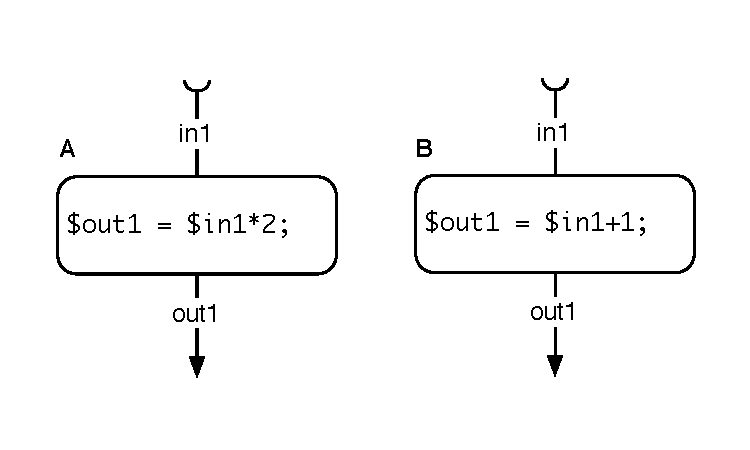
\includegraphics[width=\columnwidth]{images/code-gen1}
\caption{Two basic blocks, A and B.}
\label{fig:codegen-blocks}
\end{figure}

\subsection{Block Composition}

As mentioned above, Twig provides two fundamental binary operations on blocks. The first is the \emph{sequential composition} operator, represented by the addition symbol ($+$). Sequencing connects two blocks of code by ``wiring'' the outputs of the first block into the inputs of the second. In C, this is done by creating temporary variables which are substituted into the original blocks. For example, see Figure~\ref{fig:codegen-seq}, which builds on Figure~\ref{fig:codegen-blocks}.

\begin{figure}[ht]
\centering
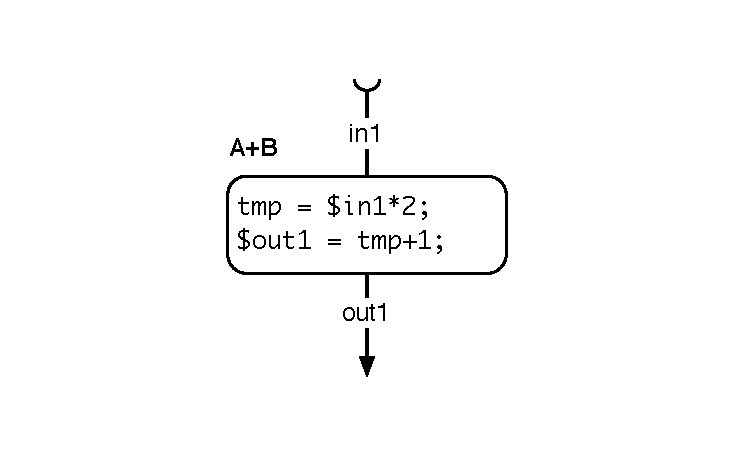
\includegraphics[width=\columnwidth]{images/code-gen2}
\caption{Two blocks from Figure~\ref{fig:codegen-blocks} composed sequentially. The variable ``tmp'' is created, and renaming performed, so that the output of block A would flow to the input of block B.}
\label{fig:codegen-seq}
\end{figure}

Twig's implementation takes care of declaring and uniquely naming temporary variables to accomplish sequencing.

The second operator is \emph{parallel composition}. Under this operator, two blocks are combined so as to execute independently of one another, but to appear as one single block. We represent this operation with the multiplication operator ($\times$). An example is shown in Figure~\ref{fig:codegen-par}.

\begin{figure}[ht]
\centering
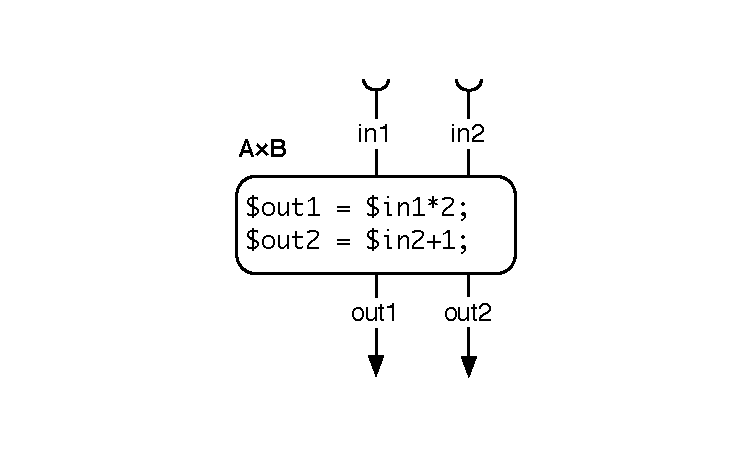
\includegraphics[width=\columnwidth]{images/code-gen3}
\caption{Two blocks from Figure~\ref{fig:codegen-blocks} composed in parallel. Renaming is performed such that the composed block has two inputs and two outputs.}
\label{fig:codegen-par}
\end{figure}

\subsection{Special Blocks}

Twig defines a special set of blocks called \emph{permutation} blocks. These blocks have some special properties, which we will exploit for the purposes of rewriting programs to remove redundant memory copies. In particular, some kinds of blocks act as a kind of identity element when composed with others.

The permutation blocks are referred to as $\Pi_m(i_1,\ldots,i_n)$, and represent the primitive operation of rearranging $m$ inputs to $n$ outputs, possibly in a different order, and possibly duplicating or dropping elements. The data is only passed through, and are otherwise unchanged.

Among the permutation blocks, there are a set of elements for which we provide special rules; namely, a set of \emph{identity} permutations. The simplest of these is $\Pi_1(1)$, which acts as an identity transformation with one input and one output. We refer to this element as $I_1$. In fact, there are an unlimited number of identity transformations, which take $n$ inputs to $n$ outputs, unchanged. These are referred to as $I_n$, where $1 \leq n$, and $I_n = \Pi_n(1,2,\ldots,n)$. The blocks $I_n$ are left- and right-identity elements under a sequence operation. We sometimes use $I_n$ as a kind of ``no-op.''

Using this simple system, a wide variety of code can be generated.

%!TEX root = twig-gpu.tex

\section{Twig}

% Overview of how Twig works, basic semantics, code generation, simple
% example. Focus on importance of generating C - integration with existing
% methods, type-directed generation.

Twig is based a core semantics called System S~\cite{Visser:1998p333}. System
S was originally designed for specifying term rewriting systems (described
briefly in \ref{section:term-rewriting}). In Twig, we use the operators of
System S to combine primitive \emph{rules} into more complex transformations
on types. These transformations are then applied to a given type in order to
generate code. In this section we describe Twig's language.

\subsection{Rules}

The basic building blocks of a Twig program are called \emph{rules}. A rule simply specifies that a given type can be transformed into another type, and provides a snippet of code which performs the transformation. The snippets are essentially strings

\subsection{Values}

Values in Twig are types in the target language.

\subsection{Combinators}

Rules can be combined into more complex expressions using a fixed set of
operators.

\subsection{Code generation}

Our implementation of Twig generates C code, but in principle almost any
language could be generated instead.

\subsection{Reductions}

Reductions are a way to transform Twig expressions. Reductions may exploit
some application or domain knowledge about the nature of the rules, and as
such are usually developed alongside a set of rules.

% Explain reductions and how they can be used in domain- or
% application-specific ways.

\subsection{Term rewriting}
\label{section:term-rewriting}

% Brief overview of term rewriting and how it is used in reductions.

\subsection{Implementation}

% Talk briefly about how Twig is implemented, and how to use it to generate
% code.

%!TEX root = twig-language.tex

\section{Evaluation}

Evaluation. 

\begin{verbatim}
%typemap(in) int {
    $1 = PyInt_AsLong($input);
}
%typemap(out) int {
    $result = PyInt_FromLong($1);
}
\end{verbatim}

\begin{verbatim}
%typemap(in) int {
    $1 = PyInt_AsLong($input);
}
%typemap(out) int {
    $result = PyInt_FromLong($1);
}
\end{verbatim}

% Show a simple example written in both Swig and Twig, and show how Twig's composition operators make the code cleaner.

%!TEX root = twig-gpu.tex

\section{Conclusion}
\label{sec:conclusion}

We have introduced the concept of separating the protocol logic that is inherent to hybrid systems from the computational logic that forms the domain specific intent of a program that uses the system. We have demonstrated that a type-based approach can enforce this separation by making explicit in data types information related to both the locale in which data resides, and the representation of the data itself. By doing so, we allow the protocol logic of a program to be expressed via operations exclusively on located types. Many explicit programming chores become implicit features of the generated code, such as declaring intermediate values or reducing redundant memory movement. Finally, by adopting a code generation approach, we show that users of these higher level abstractions are not prohibited from both tuning the resultant code and composing together independently developed programs that utilize standardized hybrid programming libraries like OpenCL or CUDA.


This work was supported in part by the Department of Energy Office of Science,
Advanced Scientific Computing Research.

% \pagebreak
\bibliographystyle{abbrv}
\bibliography{twig-language}

\end{document}
